\chapter{Cycle 2 --- Types and Pattern Matching}
In this cycle, I moved away from the autoethnographic (\ref{sec:c1_autoethnography}) approach, where most of my requirements came from within, to an externally motivated client-led approach. 

At the end of this cycle, I held a focus group (\ref{ref:afg}) to help me evaluate the progress of the project. Because this was the plan from the beginning of the cycle, 

\section{Requirements Analysis}
The requirements for this cycle were motivated by my client meeting (\ref{eval:c1}). I wanted to tackle the most technical aspects in this cycle to give me the maximum time to complete them, as this was still early in the project lifecycle. The most difficult features out of the client's requests were the ones to do with extending the language, so these were the main focus for this cycle. 

The client's central idea for what they wanted to use the tool was to demonstrate methods on lists, such as `map' and `foldr/l'. This requires lists to be built into the language. Lists in functional programming languages are commonly defined recursively, using \verb|Cons x xs| to represent constructing a list from an element \verb|x| and the rest of the list \verb|xs|. \verb|Nil| represents an empty list. This recursive construction of lists comes from Lisp \cite{mccarthy1960recursivelisp}. 

In Haskell, lists are defined as \verb!data [a] = [] | a : [a]! \\\todo{finish yapping about lists and talk about why that means we need ADTs}

\section{Design}
\subsection{Language Changes}
\subsubsection{Type System}
We must have types representing integers and booleans in our language, if we are to effectively represent the type of expression containing their respective literals. We also want our type system to be able to express functions. We also want polymorphism in our type system, as rewriting functions many times for different data types makes programs more verbose. 

Allowing for algebraic user defined data types similarly to Haskell would make the language much more expressive and much more powerful, as well as bringing it closer to Haskell. Supporting tagged unions and tuples in the \ac{SFL} type system would massively increase the ease of writing complex programs. It would also allow for complex data structures such as trees and lists. 

Type names, as well as constructor names, start with uppercase letters in Haskell. This allows them to be easily differentiated from type variables, as well as regular variables. 

First-order polymorphic type constructors would be useful to have in \ac{SFL}, with one example of their utility being defining the polymorphic function `\verb|length :: List a -> Int|' which should work regardless of what type the list is over.

\begin{figure}[h]
  \centering
  \[
      \begin{array}{llcl}
      \text{Types} & A, B, C & \bnfas &
            \Inttype \bnfalt \Booltype \bnfalt \alpha \bnfalt 
            \alltype{\alpha}{A} \bnfalt A \arr B \bnfalt
            % \\[1pt] &&&\!\!\!\;\; \TypeAlias{A}{B} \bnfalt  
            (A, B) \bnfalt
            \Unionname[A_1, \dots, A_n]
      \\[2pt]
      \text{Monotypes} & \tau,\sigma & \bnfas &
            \Inttype \bnfalt \Booltype \bnfalt \alpha \bnfalt \ahat \bnfalt 
            A \arr B \bnfalt (A, B)
            % (A, B) \bnfalt \TypeAlias{A}{B}
        \\[2pt]
      \end{array}
  \]
  
  \captionsetup{justification=centering}\caption{Syntax of types and monotypes. Note that this is the external definition: as seen by the users of SFL. See \ref{fig:tc_types} for the extra type system structures required internally for the typechecker}
  \FLabel{fig:alg-syntax}
\end{figure}

We can avoid thinking about kinds by enforcing that a type constructor is always given the correct number of arguments

% \begin{syntax}[Types in \ac{SFL}]
% (Inbuilts): \(B::=Int\mid Bool\)\newline
% (Monotype): \(\tau, \sigma ::= \alpha \mid B \mid \tau \rightarrow \sigma \mid (\tau, \sigma) \mid \Alpha \;T, U,...\)\newline
% (Alias): \(A ::= Id = T\)\newline
% (Type): \(T, U ::= \alpha \mid B \mid T \rightarrow U \mid (T, U) \mid \forall a. T \mid \Alpha \;T, U,...\)
% \end{syntax}
Note that our type constructor application definition above is more permissive than is correct, as it does not enforce correct arity. This can be handled by the parser maintaining the context of the arity of each type. It can then be double-checked for debugging purposes via an assertion in the type checker. 

\subsubsection{Match}
To support different execution based on a condition, we must have some structure that can differentiate between values.  

\subsubsection{Syntax Sugar}

\subsection{Next UI Iteration}
\label{c2:next_ui}
At this phase of the project, the current version of the web UI is a proof of concept. See \ref{fig:screenshot_cycle_1_end} for the current state. 

I completely redesigned the UI based on the clients' feedback, as well as some other factors.  See \ref{fig:screenshot_figma1} and \ref{fig:screenshot_figma2} for screenshots of the new design. These designs were done using \href{https://figma.com}{Figma}. 

\begin{figure}[h]
    \centering
    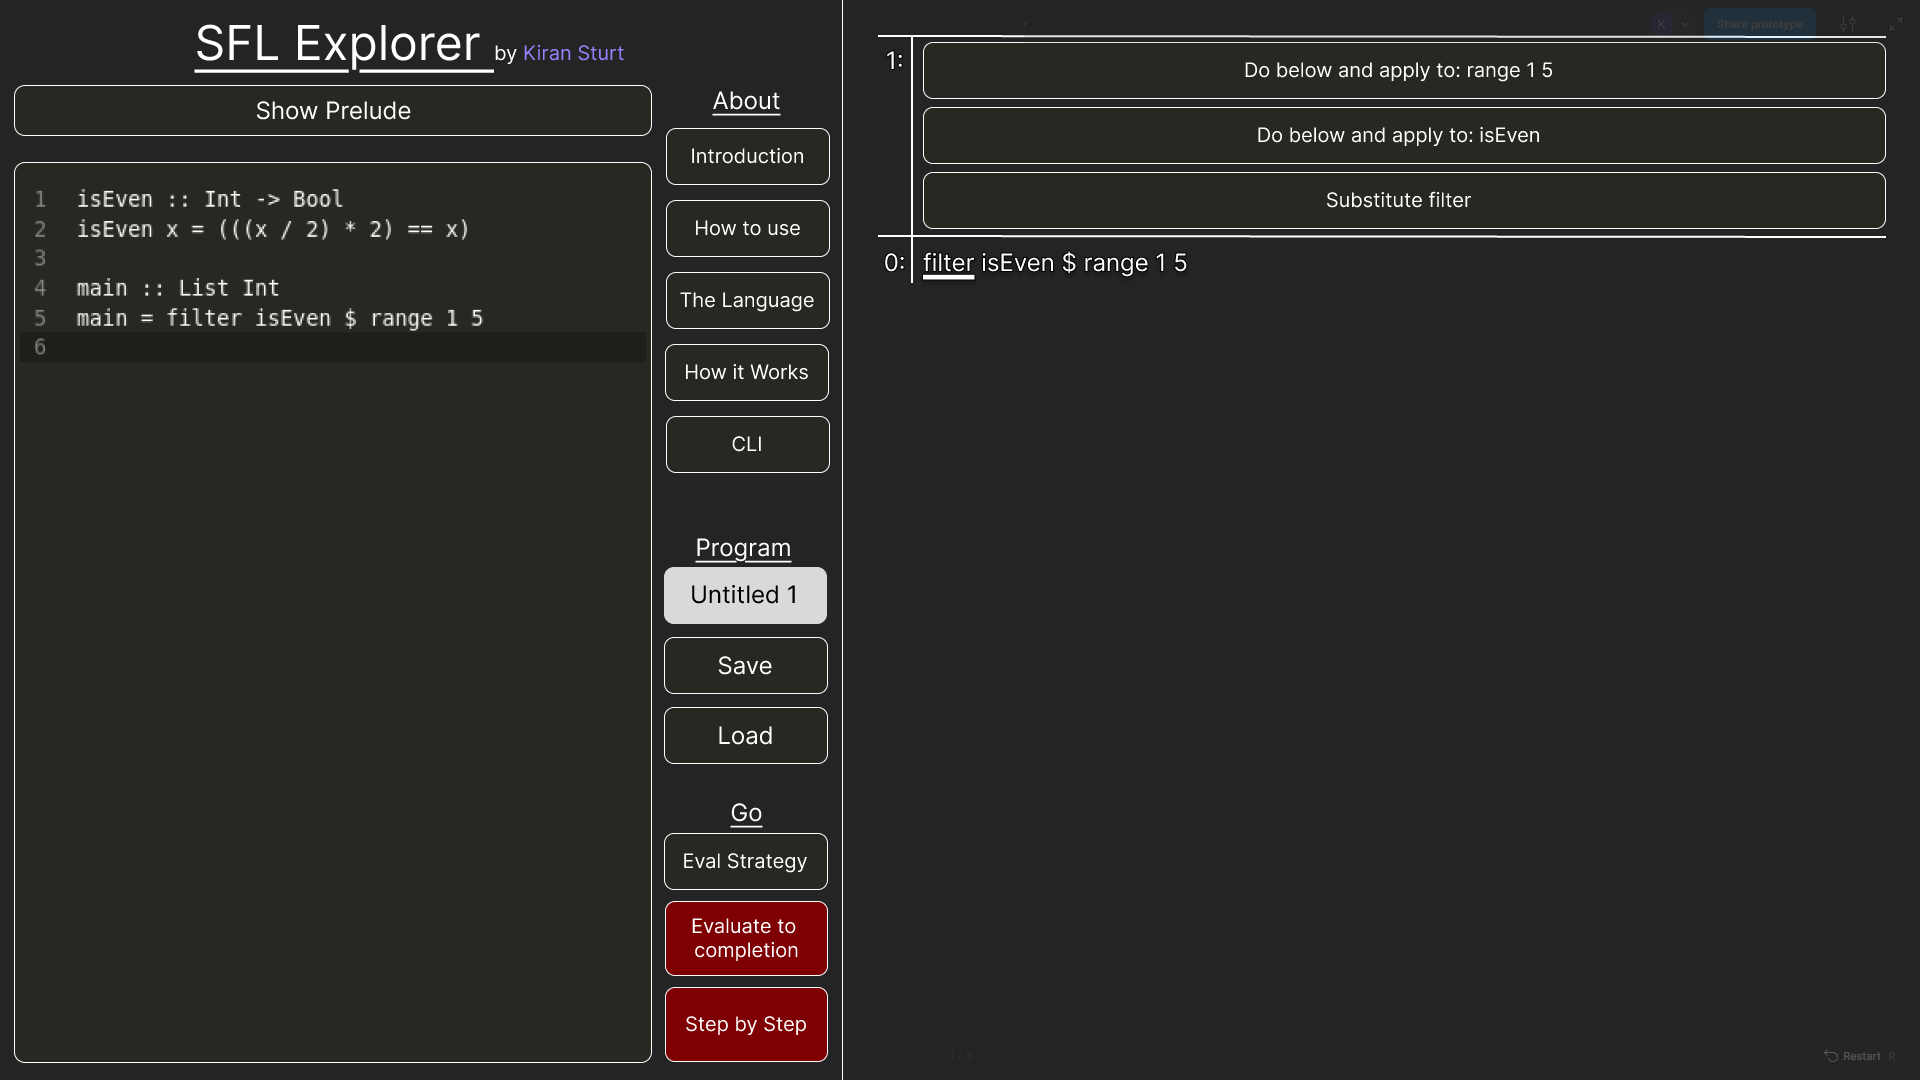
\includegraphics[width=1\linewidth]{images/figma_1.png} 
    \captionsetup{justification=centering}
    \caption{Screenshot 1 of the Figma design of the web UI}
    \label{fig:screenshot_figma1}
\end{figure}

\begin{figure}[h]
    \centering
    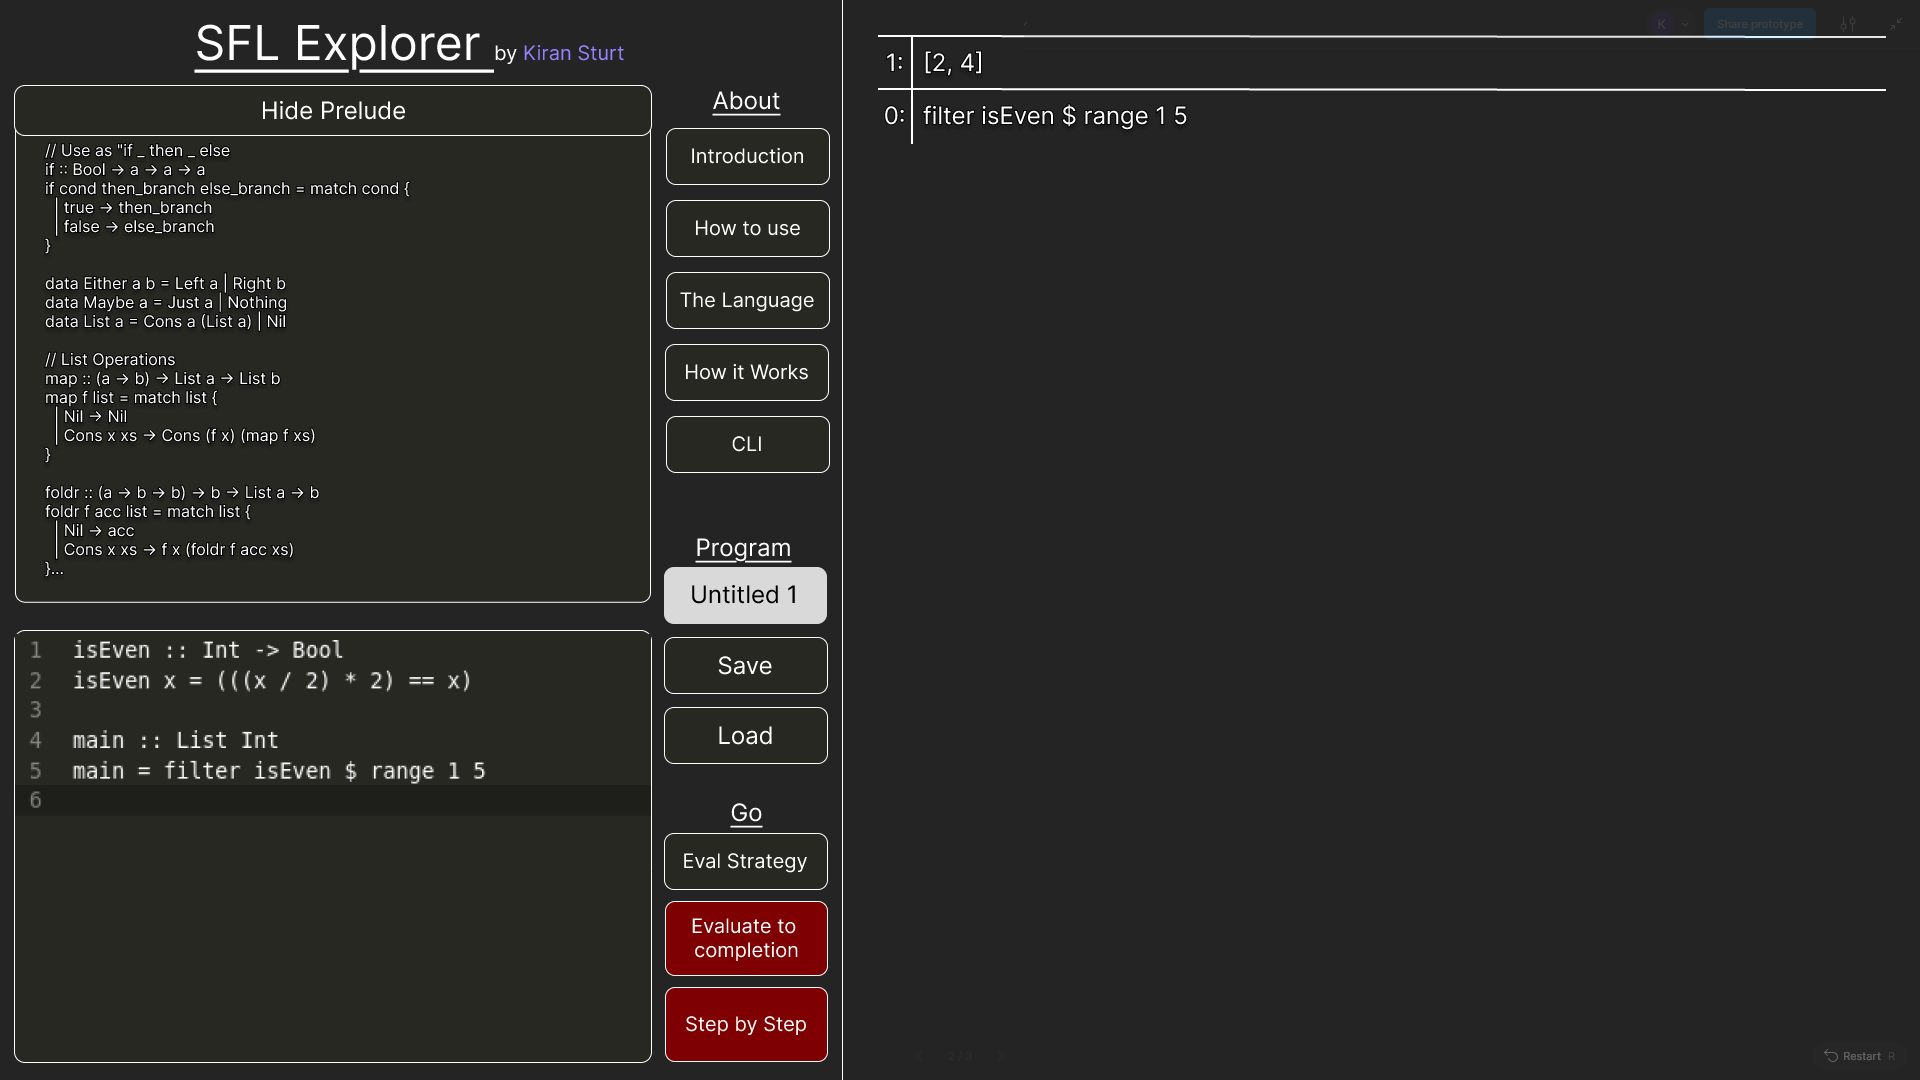
\includegraphics[width=1\linewidth]{images/figma_2.png}
    \captionsetup{justification=centering}
    \caption{Screenshot 2 of the Figma design of the web UI. This version shows the prelude extended}
    \label{fig:screenshot_figma2}
\end{figure}

This design was meant to be a work in progress, but it looks quite similar to the final release of the product (Screenshots \ref{fig:screenshot_final_dark}, \ref{fig:screenshot_final_light}, \ref{fig:screenshot_final_dark_prelude_free} and \ref{fig:screenshot_final_light_prelude_free}). Before implementing this design, I discussed this design with the Advanced Focus Group (see \ref{ref:afg_figma}) and they were much more positive about this UI than the existing one 
\todo{Discuss revert}
\todo{Design principle: simplicity, speed, minimalism, feeling like vscode.}

\section{Implementation}
\subsection{Redex Finding Changes}


\subsection{Parser Changes}
We must make some changes to the parser to include these new features.

\subsubsection{Parsing Match Statements}
An example of using a match statement follows:
\begin{verbatim}
lengthIsAtLeast2 list = match list {
  | Cons x (Cons y xs) -> true
  | _ => false
}
\end{verbatim}

The algorithm used for parsing match statements is:
\begin{itemize}
    \item Consume the `match' keyword.
    \item Parse the expression matched over
    \item Consume an open brace
    \item While the next token isn't a close brace: \begin{itemize}
        \item Parse a pattern (\ref{impl:parsing_patterns}).
        \item Consume a right arrow
        \item Parse an expression
    \end{itemize}
    \item Consume a close brace
\end{itemize}
Following this, a match node is created, where the \verb|children| vector is set appropriately with the pattern and expressions.

\paragraph{Patterns}
\label{impl:parsing_patterns}
A pattern must be a value \ref{design:values}; a pattern must not contain anything that can be reduced. It would be nonsensical to have a situation where we had a pattern not in normal form such as \verb|1 + 1| and the expression to be matched was \verb|2|. 

To parse a pattern, we may use the same techniques as parsing an expression, with a few differences:
\begin{itemize}
    \item Disallowing abstractions
    \item Identifiers must be either
    \begin{itemize}
        \item Unbound lowercase variables
        \item Underscore (\verb|_|) representing a wildcard pattern
        \item A bound uppercase variable (a constructor)
    \end{itemize}
\end{itemize}

\subsection{Types}

Rust allows us to represent our types (see \ref{fig:tc_types} for the definition of the type system), quite easily using Enums. Rust's Enums are an example of algebraic data types, and are therefore very useful for defining our own algebraic data type system. See \ref{fig:type_lst} for the listing. 

\begin{figure}[ht]
    \centering
    \begin{tabular}{|c|}
    \hline
    \begin{lstlisting}[language=Rust]
pub enum Primitive {
    Int64,
    Bool,
}

pub enum Type {
    Unit,
    Primitive(Primitive),
    Function(Box<Type>, Box<Type>),
    TypeVariable(String),
    Forall(String, Box<Type>),
    Product(Box<Type>, Box<Type>),
    Union(String, Vec<Type>),
    Alias(String, Box<Type>),

    Existential(usize),
}
    \end{lstlisting}
    \\\hline
    \end{tabular}
    \caption{The Rust code listing for the definition of types. Existential is separated as it is more of an implementation detail than a part of the type system}
    \label{fig:type_lst}
\end{figure}

We must use \verb|Box<Type>|, which represents a pointer to a heap allocated object, otherwise it would be impossible to calculate the size of \verb|Type|, as it could be infinitely large with it containing another \verb|Type| recursively. \verb|Box<Type>| however has known size: the size of a pointer in the target architecture. We also define Existential, as an implementation detail needed for the type checker. 

\subsubsection{Methods on Types}
Below are a selection of the more important or interesting methods implemented on Types.

\paragraph{Substitution of type variables} We may wish to set a type variable to another type. For instance, if given the type expression \(T \; U\) where \(T\) and \(U\) are types, and we know that one of the constructors of \(T\) is of generic type \(\forall a.a \rightarrow T \; a\), the type of the constructor for this type should be \(U \rightarrow T \; U\). We have `instantiated' the type variable \(a\) to be \(U\) by substituting \(a\) with \(U\) throughout the expression, and removing the \(\forall a\). This is required for the type checker. 

\paragraph{To String} We will frequently wish to display types as strings for debugging purposes. 

\subsection{The Type Checker}
The type checker will be bidirectional, and will follow and algorithm largely based on the one in \cite{completebidir}. The quote that follows from this paper, describes bidirectional type checking and its merits:
\begin{quote}
`Bidirectional typechecking, in which terms either synthesize a type or are checked against a known type, has become popular for its scalability \ldots its error reporting, and its relative ease of implementation' \cite{completebidir}
\end{quote}
\noindent It was the `relative ease of implementation' that attracted me to bidirectional type checking. After running the algorithm by hand to convince myself the algorithm works on checking id ($\lambda x. x$) against type $\forall a.a\fto a$ (photo of whiteboard derivation included in submission [TODO: is this the right way to cite this]), I modified their algorithm to add my extra types (The inbuilt types $Int$, $Bool$, as well as the \Uniontype\ and \Producttype\ types) and my extra expression syntax structures (literals, match, pairs. Not including assignment and modules as these are not part of expression syntax). \ref{fig:tc_types} shows the type system, including the typechecker implementation details, as well as the unmodified context structure, which keeps track of the state of the typechecker as it progresses recursively through the type system. \ref{appx:example_derive} shows some example derivations using this algorithm including some of my rules. \ref{fig:ctx_subst} shows the modified algorithm for substituting all of the information in a context into a type. 

\begin{figure}[h]
  \centering
  \begin{minipage}{\textwidth}
  \[
      \begin{array}{llcl}
      % \\[4pt]
      \text{Types} & A, B, C & \bnfas &
            \Inttype \bnfalt \Booltype \bnfalt \alpha \bnfalt \ahat \bnfalt 
            % \\[1pt] &&&\!\!\!\;\;\;
            \alltype{\alpha}{A} \bnfalt A \arr B \bnfalt
            % \\[1pt] &&&\!\!\!\;\; \TypeAlias{A}{B} \bnfalt  
            % \\[1pt] &&&\!\!\!\;\;
            (A, B) \bnfalt
            % \\[1pt] &&&\!\!\!\;\;
            \Unionname[A_1, \dots, A_n]
      \\[2pt]
      \text{Monotypes} & \tau,\sigma & \bnfas &
            \Inttype \bnfalt \Booltype \bnfalt \alpha \bnfalt \ahat \bnfalt 
            % \\[1pt] &&&\!\!\!\;\;
            \tau \arr \sigma \bnfalt (\tau, \sigma) \bnfalt \Unionname[\tau_1, \dots, \tau_n]
            % (A, B) \bnfalt \TypeAlias{A}{B}
        \\[2pt]
      \text{Contexts} & \Gamma, \Delta, \Theta & \bnfas &
                  \cdot
                  \bnfalt \Gamma, \alpha 
                  \bnfalt \Gamma, x:A
                  % \\[1pt] &&&\!\!\!\;\;
                  \bnfalt \Gamma, \ahat
                  \bnfalt \Gamma, \hypeq{\ahat}{\tau}
                  % \\[1pt] &&&\!\!\!\;\;
                  \bnfalt \Gamma, \MonnierComma{\ahat}
      % \\[2pt] % No need as I am not proving completeness
      % \text{Complete Contexts}     & \Omega & \bnfas &
      %             \cdot
      %             \bnfalt    \Omega, \alpha
      %             \bnfalt    \Omega, x:A
      %             \\[1pt] &&&\!\!\!
      %             \bnfalt    \Omega, \hypeq{\ahat}{\tau} 
      %             \bnfalt    \Omega, \MonnierComma{\ahat}
      \end{array}
  \]
  
  \captionsetup{justification=centering}\caption{Syntax of types, monotypes, and contexts as seen by the typechecker. The definition of types differ slightly from the definition offered in figure \ref{fig:sfl_types_no_exst}, as we include existential type variables ($\ahat$) that can not actually be created by users. They are an implementation detail required for the type checking algorithm}
  \FLabel{fig:tc_types}

  
  \end{minipage}
  \hfill
  \begin{minipage}{\textwidth}
    \centering
      \[
  \begin{array}[t]{l@{~}c@{~}ll}
      %
      [\Gamma]\Inttype  & = & \Inttype &\\{}

      [\Gamma]\Booltype & = & \Booltype &\\{}

      [\Gamma]\alpha    & = & \alpha &\\{}
      % [\Gamma]\unitty   & = &   \unitty &
      % \\[1pt]
      \big[\Gamma[\hypeq{\ahat}{\tau}]\big] \ahat
               & = &   \big[\Gamma[\hypeq{\ahat}{\tau}]\big]\tau &
      \\[2pt]
      \big[\Gamma[\ahat]\big]\ahat   & = &   \ahat &
      \\[2pt]
      [\Gamma](A \arr B)   & = &
          ([\Gamma]A) \arr ([\Gamma]B) &
      \\{}
      [\Gamma](\alltype{\alpha} A)
         & = & 
         \alltype{\alpha} [\Gamma]A &
      \\[2pt]
      [\Gamma](A, B) 
         & = &
         ([\Gamma]A, [\Gamma]B)
      \\[2pt]
      [\Gamma]\Unionname[A_1,\dots, A_n]
         & = &
         \Unionname[[\Gamma]A_1,\dots, [\Gamma]A_n]
  \end{array}
  \]
  \captionsetup{justification=centering}\caption{Applying a context, as a substitution, to a type}
  \FLabel{fig:ctx_subst}
  \end{minipage}
\end{figure}


The full typechecking algorithm is listed in figures \ref{fig:alg-subtyping}, \ref{fig:instantiation}, \ref{fig:alg-typing}. \ref{fig:alg-typing} shows the main algorithm for checking and synthesizing the types of various expression structures. \ref{fig:alg-subtyping} shows the algorithm for how we verify that a type is a subtype of another type. For instance, our typechecking rule $\Sub$ synthesizes the type, and the uses the algorithmic subtyping rules to check that the synthesized type is a subtype of the expected type. 

Most of these rules are untouched, the ones that I added or modified are \colorbox{myTcRuleColour}{highlighted}.


\begin{figure*}[htbp]
  \judgbox{\subjudg{\Gamma}{A}{B}{\Delta}}%
     {Under input context $\Gamma$,
       type $A$ is a subtype of $B$, with output context $\Delta$}
  \begin{mathpar}
  \Infer{\SubVar}
              { }
              {\subjudg{\Gamma[\alpha]}{\alpha}{\alpha}{\Gamma[\alpha]}}
  \and
  \Infer{\MyTCRule{\Intsubrulename}}
            { }
            {\subjudg{\Gamma}{\Inttype}{\Inttype}{\Gamma}}
              \and
  \Infer{\MyTCRule{\Boolsubrulename}}
            { }
            {\subjudg{\Gamma}{\Booltype}{\Booltype}{\Gamma}}
  \\
  % \Infer{\MyTCRule{\LAliassubrulename}}
  %           { \subjudg{\Gamma}{C}{B}{\Delta}  }
  %           { \subjudg{\Gamma}{\TypeAlias{A}{C}}{B}{\Delta} }
  % \and
  %   \Infer{\MyTCRule{\RAliassubrulename}}
  %           { \subjudg{\Gamma}{A}{C}{\Delta}  }
  %           { \subjudg{\Gamma}{A}{\TypeAlias{B}{C}}{\Delta} }
  % \\
  \Infer{\SubExvar}
            { }
            {\subjudg{\Gamma[\ahat]}{\ahat}{\ahat}{\Gamma[\ahat]}}
  \and
  \Infer{\SubArr}
            {\subjudg{\Gamma}{B_1}{A_1}{\Theta} \\
              \subjudg{\Theta}{[\Theta]A_2}{[\Theta]B_2}{\Delta}}
            {\subjudg{\Gamma}{A_1 \arr A_2}{B_1 \arr B_2}{\Delta}}
  \\
  \Infer{\SubAllL}
            {\subjudg{\Gamma, \MonnierComma{\ahat}, \ahat}
                     {[\ahat/\alpha]A}
                     {B}
                     {\Delta, \MonnierComma{\ahat}, \Theta}}
            {\subjudg{\Gamma}{\alltype{\alpha}{A}}{B}{\Delta}}
  \and
  \Infer{\SubAllR}
            {\subjudg{\Gamma, \alpha}{A}{B}{\Delta, \alpha, \Theta}}
            {\subjudg{\Gamma}{A}{\alltype{\alpha}{B}}{\Delta}}
  \\
  \Infer{\SubInstL}
            {
              \ahat \notin \FV{%
                A}
              \\
              \instjudg{\Gamma[\ahat]}{\ahat}{%
                   A}{\Delta}
            }
            {\subjudg{\Gamma[\ahat]}{\ahat}{A}{\Delta}}
  \and
  \Infer{\SubInstR}
            {
              \ahat \notin \FV{%
                A}
              \\
              \instjudgr{\Gamma[\ahat]}{\ahat}{%
                A}{\Delta}
            }
            {\subjudg{\Gamma[\ahat]}{A}{\ahat}{\Delta}}
  \\
  \Infer{\MyTCRule{\Pairsubrulename}}
    {\subjudg{\Gamma}{A_1}{A_2}{\Theta} \\
              \subjudg{\Theta}{B_1}{B_2}{\Delta}}
    { \subjudg{\Gamma}{(A_1, B_1)}{(A_2, B_2)}{\Delta} }
      \\
  \Infer{\MyTCRule{\Unionsubrulename}}
    {(\subjudg{\Gamma_i}{A_i}{B_i}{\Gamma_{i+1}})\;\tcforin{i}{[1, 2, \dots, n]}}
    {\subjudg{\Gamma_1}{\Unionname[A_1, A_2, \dots, A_n]}{\Unionname[B_1, B_2, \dots, B_n]}{\Gamma_{n+1}}}
  \end{mathpar}  
  \caption{Algorithmic subtyping. The rules with \colorbox{myTcRuleColour}{highlighted} names are my additions, the rest are unchanged from \cite{completebidir}}
  \FLabel{fig:alg-subtyping}
\end{figure*}


\begin{figure*}[h]
      \judgbox{\instjudg{\Gamma}{\ahat}{A}{\Delta}}%
         {Under input context $\Gamma$,
           instantiate $\ahat$ such that $\ahat \subtype A$, 
           with output context $\Delta$}
      \begin{mathpar}
        \Infer{\InstLSolve}
                { \Gamma \entails \tau} %
                { \instjudg{\Gamma, \ahat, \Gamma'}
                            {\ahat}
                            {\tau}
                            {\Gamma, \hypeq{\ahat}{\tau}, \Gamma'}
                 }
        \and
        \Infer{\InstLReach}
                { }
                {\instjudg{\Gamma[\ahat][\bhat]}
                            {\ahat}
                            {\bhat}
                            {\Gamma[\ahat][\hypeq{\bhat}{\ahat}]}}
        \and
        \Infer{\InstLArr}
                {\instjudgr{\Gamma[\ahat_2, \ahat_1, \hypeq{\ahat}{\ahat_1 \arr \ahat_2}]}
                            {\ahat_1}
                            {A_1}
                            {\Theta} \\
                 \instjudg{\Theta}
                            {\ahat_2}
                            {[\Theta]A_2}
                            {\Delta}}
                {\instjudg{\Gamma[\ahat]}
                            {\ahat}
                            {A_1 \arr A_2}
                            {\Delta}}
        \and
        \Infer{\InstLAllR}
              {\instjudg{\Gamma[\ahat], \beta}{\ahat}{B}{\Delta, \beta, \Delta'}}
              {\instjudg{\Gamma[\ahat]}{\ahat}{\alltype{\beta}{B}}{\Delta}}
      \end{mathpar}    
    %
    \\[-1.5ex]
    %
      \judgbox{\instjudgr{\Gamma}{\ahat}{A}{\Delta}}
         {Under input context $\Gamma$,
           instantiate $\ahat$ such that $A \subtype \ahat$,
           with output context $\Delta$}
      \small\begin{mathpar}
        \Infer{\InstRSolve}
                { \Gamma \entails \tau}
                { \instjudgr{\Gamma, \ahat, \Gamma'}
                            {\ahat}
                            {\tau}
                            {\Gamma, \hypeq{\ahat}{\tau}, \Gamma'}
                 }
        \and
        \Infer{\InstRReach}
                { }
                {\instjudgr{\Gamma[\ahat][\bhat]}
                           {\ahat}
                           {\bhat}
                           {\Gamma[\ahat][\hypeq{\bhat}{\ahat}]}}
        \and
        \Infer{\InstRArr}
              {\instjudg{\Gamma[\ahat_2, \ahat_1, \hypeq{\ahat}{\ahat_1 \arr \ahat_2}]}
                        {\ahat_1}
                        {A_1}
                        {\Theta} \\
                 \instjudgr{\Theta}
                           {\ahat_2}
                           {[\Theta]A_2}
                           {\Delta}}
              {\instjudgr{\Gamma[\ahat]}
                         {\ahat}
                         {A_1 \arr A_2}
                         {\Delta}}
        \and 
        \Infer{\InstRAllL}
              {\instjudgr{\Gamma[\ahat], \MonnierComma{\bhat}, \bhat}{\ahat}{[\bhat/\beta]B}{\Delta, \MonnierComma{\bhat}, \Delta'}}
              {\instjudgr{\Gamma[\ahat]}{\ahat}{\alltype{\beta}{B}}{\Delta}}
      \end{mathpar}

\caption{Instantiation}
\FLabel{fig:instantiation}
\end{figure*}
\begin{figure*}[ht]
  \judgbox{\chkjudg{\Gamma}{e}{A}{\Delta}}%
     {Under input context $\Gamma$, $e$ checks against input type $A$, 
     with output context $\Delta$} \\[1ex]
  \judgbox{\synjudg{\Gamma}{e}{A}{\Delta}}%
     {Under input context $\Gamma$, $e$ synthesizes output type $A$,
       with output context $\Delta$} \\[0.5ex]
  \judgbox{\appjudg{\Gamma}{e}{A}{C}{\Delta}}%
     {Under input context $\Gamma$, applying a function of type $A$ to $e$ synthesizes type $C$, \\ with output context $\Delta$} \\
  \begin{mathpar}
    \Infer{\MyTCRule{\Intcheckrulename}}
        { }
        {\chkjudg{\Gamma}{Int Literal}{\Inttype}{\Gamma}}
    \and
    \Infer{\MyTCRule{\Intsynthrulename}}
        { }
        {\synjudg{\Gamma}{Int Literal}{\Inttype}{\Gamma}}
    \\
    \Infer{\MyTCRule{\Boolcheckrulename}}
        { }
        {\chkjudg{\Gamma}{Bool Literal}{\Booltype}{\Gamma}}
    \and
    \Infer{\MyTCRule{\Boolsynthrulename}}
        { }
        {\synjudg{\Gamma}{Bool Literal}{\Booltype}{\Gamma}}
    \\
    \Infer{\MyTCRule{\Paircheckrulename}}
        {\chkjudg{\Gamma}{e_1}{A}{\Theta} \\ \chkjudg{\Theta}{e_2}{B}{\Delta}}
        {\chkjudg{\Gamma}{(e_1, e_2)}{(A, B)}{\Delta}}
        \and 
      \Infer{\MyTCRule{\Pairsynthrulename}}
        {\synjudg{\Gamma}{e_1}{A}{\Theta} \\ \synjudg{\Theta}{e_2}{B}{\Delta}}
        {\synjudg{\Gamma}{(e_1, e_2)}{(A, B)}{\Delta}}
     \\
     \Infer{\Var}
          {(x : A) \in \Gamma}
          {\synjudg{\Gamma}{x}{A}{\Gamma}}
      \and
    %  \Infer{\MyTCRule{\Aliasrulename}}
    %     {\chkjudg{\Gamma}{e}{B}{\Delta}}
    %     {\chkjudg{\Gamma}{e}{[A : B]}{\Delta}}
    % \and
     \Infer{\Sub}
          {\synjudg{\Gamma}{e}{A}{\Theta}
            \\
            \subjudg{\Theta}{[\Theta]A}{[\Theta]B}{\Delta}
          }
          {\chkjudg{\Gamma}{e}{B}{\Delta}}
      \\ 
     \def\CompactJudgments{1}   %
     \Infer{\AllIntro}
           {\chkjudg{\Gamma, \alpha}{e}{A}{\Delta, \alpha, \Theta}
           }
           {\chkjudg{\Gamma}{e}{\alltype{\alpha}{A}}{\Delta}}
     \and
     \Infer{\AllApp}
            {\appjudg{\Gamma,\ahat}{e}{[\ahat/\alpha]A}{C}{\Delta}}
            {\appjudg{\Gamma}{e}{\alltype{\alpha}{A}}{C}{\Delta}}
    \and
     \Infer{\!\ArrIntro}
          {\chkjudg{\Gamma, x : A}{e}{B}{\Delta, x : A, \Theta}
          }
          {\chkjudg{\Gamma}{\lam{x} e}{A \arr B}{\Delta}}
     \\
\def\CompactJudgments{0}   %
     \Infer{%
        {\!\ArrIntroSyn}
         }
           { \chkjudg{\Gamma, \ahat, \bhat, x : \ahat}{e}{\bhat}{\Delta, x : \ahat, \Theta}
           }
           {{\synjudg{\Gamma}{\lam{x} e}{\ahat \arr \bhat}{\Delta}}}
     \and
     \Infer{\!\ArrElim}
           {\synjudg{\Gamma}{e_1}{A}{\Theta}
             \\
             \appjudg{\Theta}{e_2}{[\Theta]A}{C}{\Delta}
           }
           {\synjudg{\Gamma}{e_1\,e_2}{C}{\Delta}}
      \\
\def\CompactJudgments{0}
      %
      \Infer{\SolveApp}
            {\chkjudg{\Gamma[\ahat_2, \ahat_1, \hypeq{\ahat}{\ahat_1 \arr \ahat_2}]}{e}{\ahat_1}{\Delta}}
            {\appjudg{\Gamma[\ahat]}{e}{\ahat}{\ahat_2}{\Delta}}
      \and
      \Infer{\ArrApp}
            {\chkjudg{\Gamma}{e}{A}{\Delta}}
            {\appjudg{\Gamma}{e}{A \arr C}{C}{\Delta}}
      \\
      \Infer{\MyTCRule{\Matchsynthrulename}}
            {
            % Change to for all
            % Add footnote
            \synjudg{\Gamma}{e}{A}{\Theta_1} \\ 
            (\chkjudg{\Theta_i}{c_i}{A}{\Theta_{i+1}})\; \tcforin{i}{[1, 2, \dots, n]} \\
            \Delta_1 = \Theta_{n+1}, \ahat \\
            (\chkjudg{\Delta_{i}}{e_i}{\ahat}{\Delta_{i+1}})\; \tcforin{i}{[1, 2, \dots, n]}
            }
            {\synjudg{\Gamma}{\text{match e \{} c_1 \rightarrow e_1 \mid c_2 \rightarrow e_2 \mid \dots \mid c_n \rightarrow e_n \}}{\ahat}{\Delta_{n+1}}}
    
  \end{mathpar}
  \caption{Algorithmic typing. The rules with highlighted names are my additions, the rest are unchanged from \cite{completebidir}. }
  \FLabel{fig:alg-typing}
  \noindent\hrulefill
\end{figure*}


\pagebreak % To force the typing stuff to be on the same page

\subsection{The Prelude, and `if e then a else b'}
Most programming languages come with functionality packaged that is included by default, and is written in the language. In Haskell, this is referred to as the Prelude. There is also the standard library which is more extensive and is not imported by default. 

As our language does not need extensive extra functionality, we do not need a whole standard library. However, a basic prelude with common functionality would be useful. \ref{appx:prelude} shows the SFL prelude. I included `if' in the prelude to show that it is based on a match statement, rather than being a mysterious inbuilt: 

\begin{lstlisting}[language=SFL]
if :: Bool -> a -> a -> a
if cond then_branch else_branch = match cond {
    | true -> then_branch
    | false -> else_branch
}    
\end{lstlisting}

In order to make the language more like Haskell, I also added syntax sugar that allowed you to use it using the `\lstinline[language=SFL_ite]|if e then a else b|' syntax. The parser would ignore the `\lstinline[language=SFL_ite]|then|' and the `\lstinline[language=SFL_ite]|else|' keywords, and it would be equivalent to `\lstinline[language=SFL_ite]|(((if e)  a)  b)|' internally. However, this was unpopular with the advanced focus group, who said that this was confusing (see \ref{ref:afg_ite}). 

\subsection{Changes to the Proof of Concept UI}
\label{c2_poc_ui_impl}
In this cycle, I made some changes to the proof of concept web UI

- Initial approach to diff
- separate lazy and free choice mode

\begin{figure}[h]
    \centering
    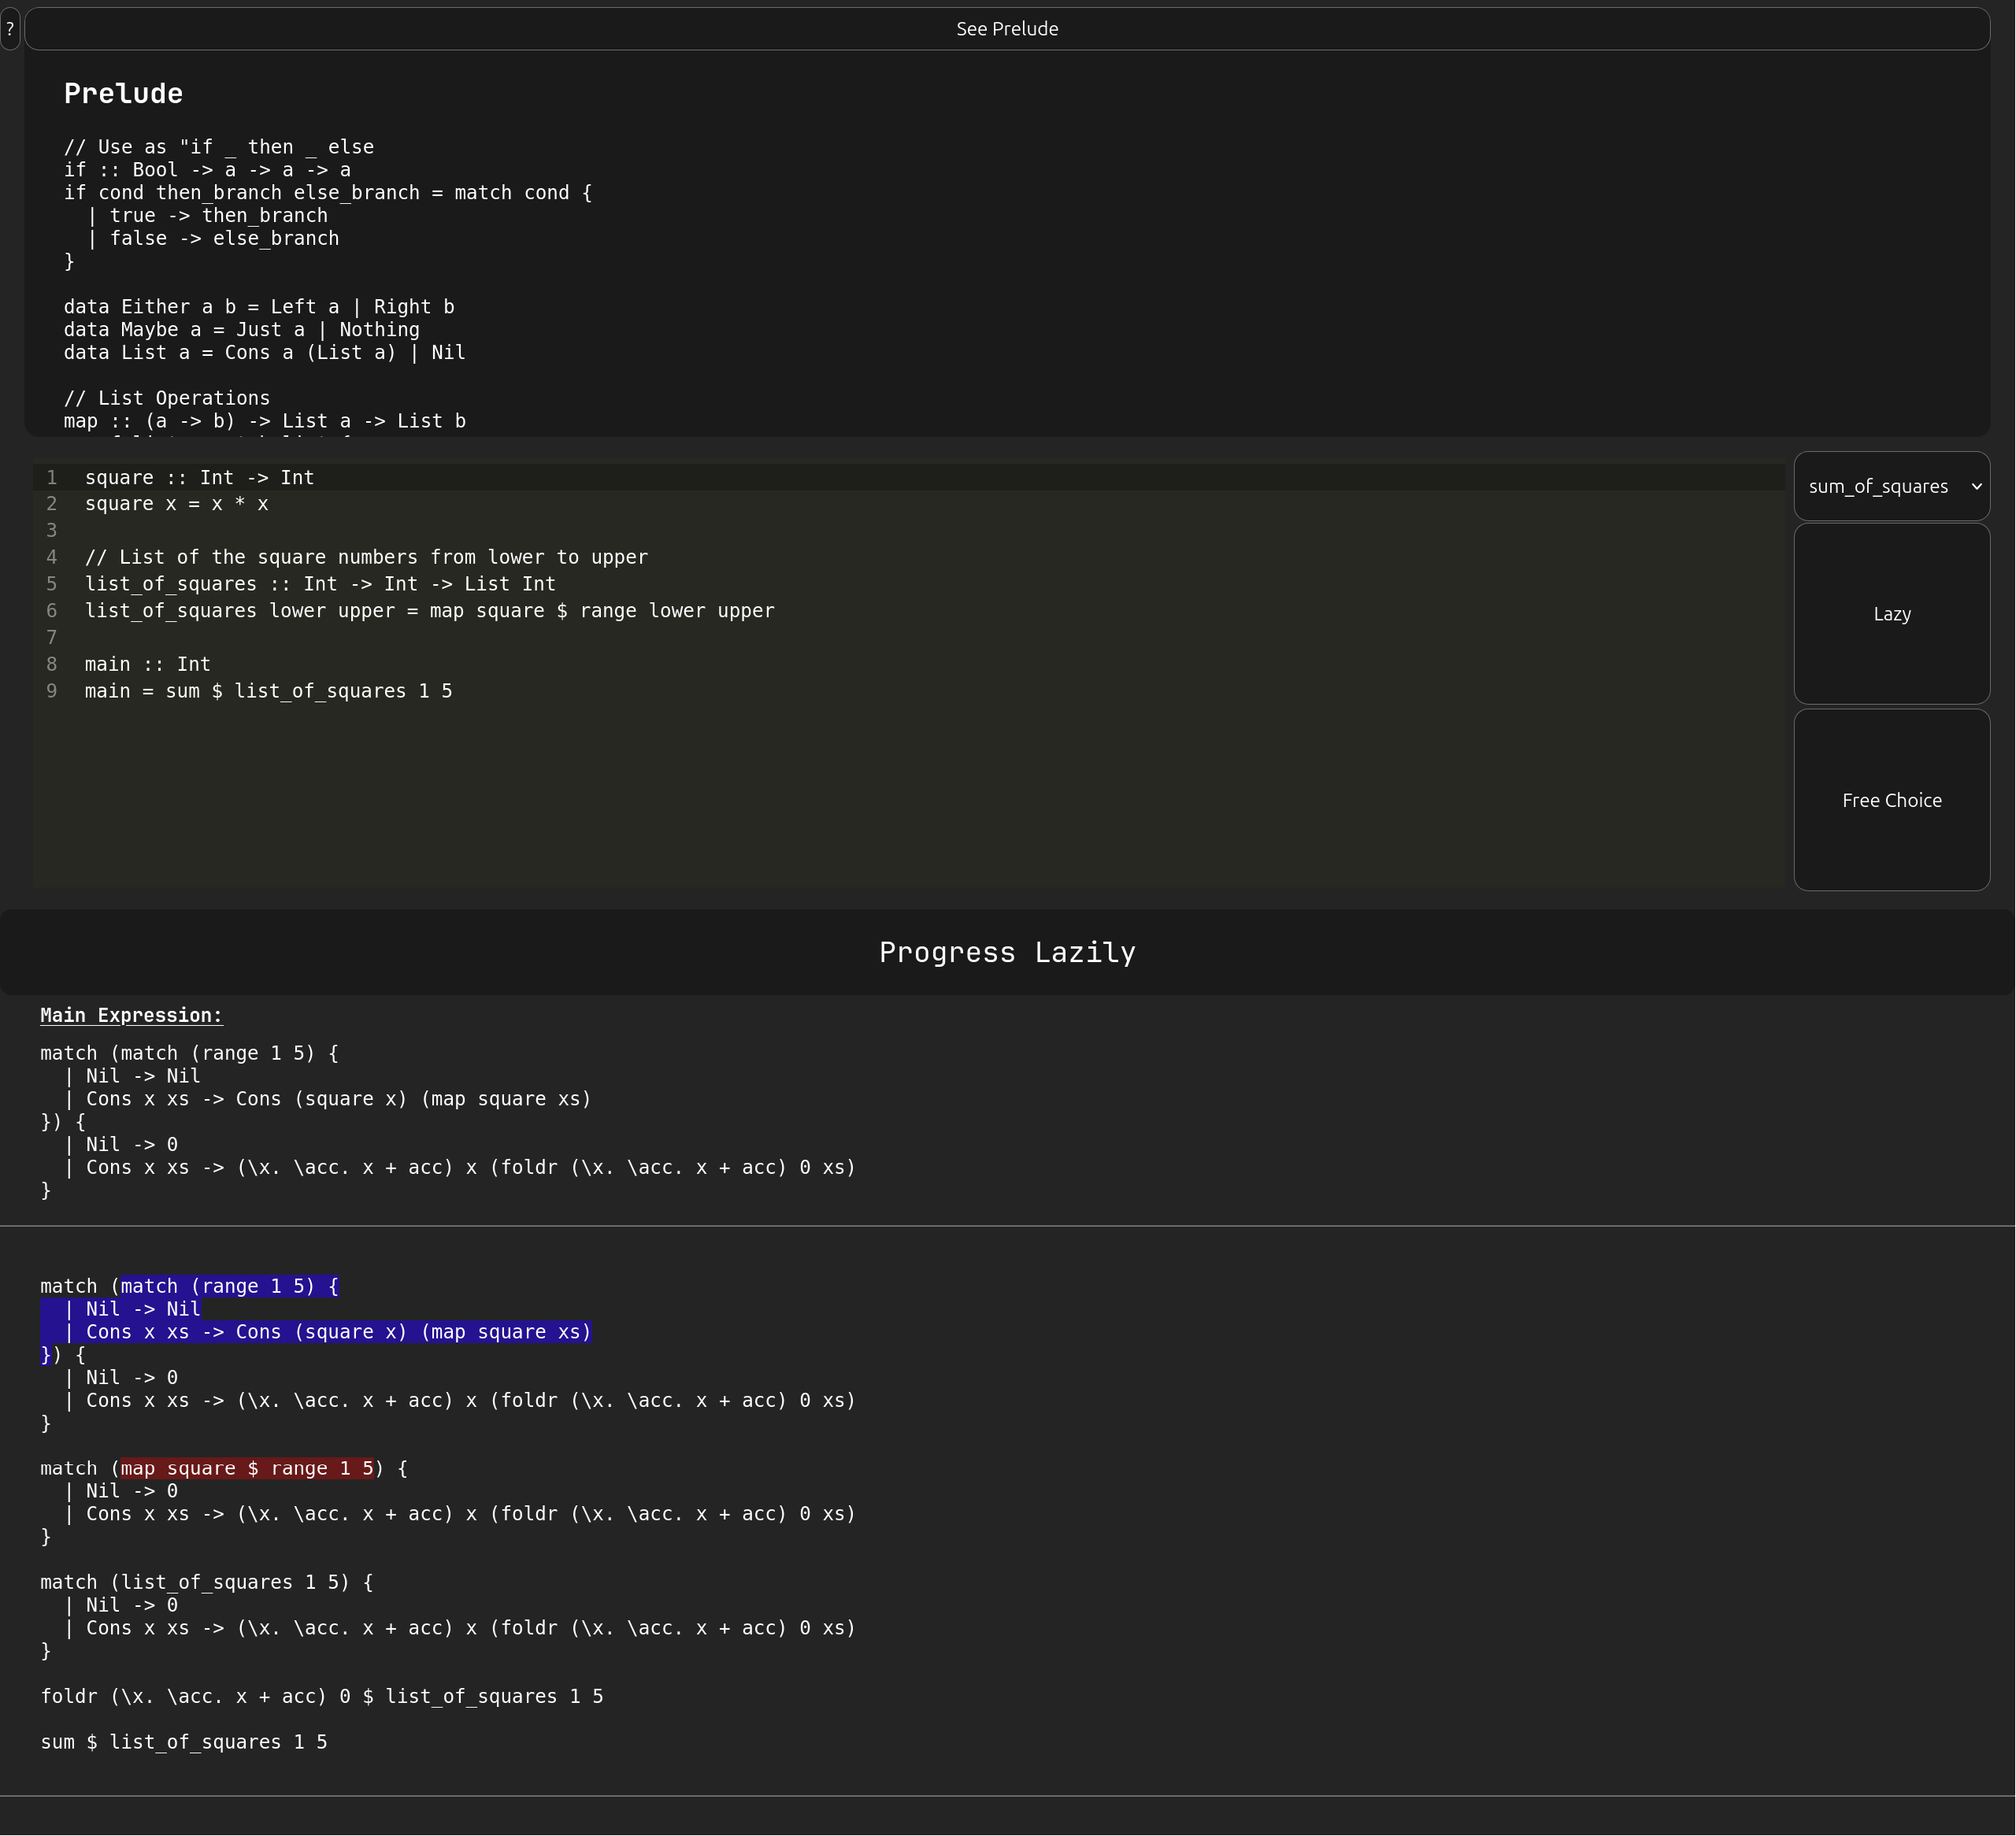
\includegraphics[width=1\linewidth]{images/cycle-2-end2.png} 
    \captionsetup{justification=centering}
    \caption{The product at the end of cycle two during lazy evaluation of the `sum of squares' sample program, with the prelude dropdown extended}
    \label{fig:screenshot_c2_end}
\end{figure}

\section{The Advanced Focus Group: Evaluation and Next Steps}
\label{ref:afg_figma}
\label{ref:afg}
The aims of this cycle were to develop the language as well as some other more technical features of this project. To discuss the language, I held a focus group with students who were very knowledgable and interested in functional programming languages. 

This was my first of three focus groups, the most advanced of the three. As the UI/UX was not polished at this stage, I wanted to find people who would be able to discuss the parts that I had already implemented to a reasonable level of completion: the language. However, I still wanted to discuss future steps for the system as a whole, rather than just the language. Because of this, I wanted to find people who had learned functional languages as a part of a university course fairly recently and within memory, so they would have an insight into what is required for the system to be useful for use in this setting. 

The transcript from this focus group is included in the additional submitted materials (see \ref{appx:additional_mats})

\subsection{Selection}

For this focus group, I recruited four students in their fourth year of studies here at the University of Bristol. They had all taken \hyperref[COMS10016]{the first-year FP unit} 3 years prior, and they had all taken units specializing in programming language theory since, including:

\begin{itemize}
    \item The second year Programming Languages and Computation unit COMS20007, where they learnt to (among other things) `Understand the interplay between the design and implementation of programming languages' \cite{COMS20007_PLC}
    \item The third year optional Types and Lambda Calculus unit COMS30040 where they learnt (among other things): \cite{COMS30040_TLC} 
    \begin{itemize}
        \item `Type systems: types, judgements and rules'
        \item `Syntax and semantics of an untyped lambda calculus'
    \end{itemize}
    \item The fourth year optional Advanced Topics in Programming Languages, where the unit outcomes were that they should be able to (among other things): \cite{COMSM0067_ATPL}
    \begin{itemize}
        \item `Specify the dynamics of program evaluation for a variety of programming constructs'
        \item `Specify static typing rules for a variety of programming constructs'
    \end{itemize}
\end{itemize}

These people I selected for this focus group were the closest to `subject experts' that I could find while still being students. 

\subsection{Format}
This focus group started with me briefly presenting SFL explorer. \ref{fig:screenshot_c2_end} shows how the system looked at this stage of the project. We also discussed the next UI iteration (see \ref{c2:next_ui}). 

\subsection{Outcomes}
Below is the summary of outcomes from the discussion with this focus group. The assertions about what they thought are backed up with quotes, marked with timestamps of where these quotes can be found in the transcript. 

\subsection{The Existing Language}
\paragraph{Positives:}
\begin{itemize}
    \item They liked the explicit match statements: `Stick with the match expressions because it's very clear that matching has happened when you have the word match there' [24:11]
\end{itemize}

\paragraph{Negatives:}
\begin{itemize}
    \item \label{ref:afg_ite} They were confused about if-then-else syntax. They said it could be confusing to have the parser act differently for one specific function type. `The issue I was having is just the fact that there is a function in the prelude which has the same name as some syntactic sugar that is a parser construct' [42.55]
\end{itemize}

\paragraph{Requested Features:}
Below are the specific features my client asked for in order for the system to be able to demonstrate the things she wants to use the system to demonstrate:
\begin{itemize}
    \item Recursive Types
    \item Polymorphism
    \item Type Aliases
    \item Typechecking
    \item User Definable Data Types
\end{itemize}

\begin{itemize}
    \item They liked the revert: `Something I had not thought of, very good' [54:59]
    \item They wanted syntax highlighting
    \item They wanted an indication of which direction evaluation was going so I added numbers: `Because the reduction steps generate bottom-up, it might be good to have some sort of indication about the direction things are going in'. This was already in the new UI, which that had not seen by this point in the transcript.
    \item They really appreciated its utility for what it was designed for. `I think this is very good \ldots\ I wish I'd had this in the functional labs' [1:00:09]
\end{itemize}

\begin{itemize}
    \item They liked the horizontal split: ` It's easier to have everything on screen and it's more akin to what people may have experienced' `Its like compiler explorer'. [52:38] `I think immediately not having to scroll is a massive plus' [52:58]
\end{itemize}